\documentclass[11pt,a4paper]{article}
\usepackage{fontspec}
\setmainfont{Liberation Sans}
\setsansfont{Liberation Sans}
\setmonofont{Liberation Mono}[Scale=0.9]
\usepackage[margin=0.95in]{geometry}
\usepackage{amsmath,amssymb}
\usepackage{booktabs,array,tabularx}
\usepackage{enumitem}
\usepackage{xcolor}
\usepackage{tikz}
\usetikzlibrary{positioning,arrows.meta,shapes.geometric}
\usepackage[hidelinks]{hyperref}
\usepackage{titlesec}
\usepackage{fancyhdr}
\usepackage{tcolorbox}

\definecolor{accent}{HTML}{1F3A5F}
\definecolor{soft}{HTML}{EEF2F7}
\setlist{nosep,leftmargin=1.3em,itemsep=2pt}
\setlist[itemize,2]{leftmargin=1.2em}
\setlength{\parindent}{0pt}
\setlength{\parskip}{5pt}
\renewcommand{\arraystretch}{1.18}
\setcounter{secnumdepth}{3}
\titleformat{\section}{\Large\bfseries\color{accent}}{\thesection.}{0.6em}{}[\vspace{-4pt}\color{accent}\rule{\linewidth}{0.6pt}]
\titleformat{\subsection}{\large\bfseries}{\thesubsection}{0.5em}{}
\titlespacing*{\section}{0pt}{16pt}{8pt}
\titleformat{\subsubsection}{\normalsize\bfseries}{\thesubsubsection}{0.5em}{}
\titlespacing*{\subsubsection}{0pt}{8pt}{2pt}
\titlespacing*{\subsection}{0pt}{10pt}{3pt}
\pagestyle{fancy}\fancyhf{}
\renewcommand{\headrulewidth}{0.3pt}
\fancyhead[L]{\small Aether: Reference-Choice Robustness}
\fancyhead[R]{\small Project Report}
\fancyfoot[C]{\small\thepage}
\newcommand{\E}[1]{E_{#1}}
\newtcolorbox{keybox}[1][]{colback=soft,colframe=accent,boxrule=0.5pt,arc=2pt,left=7pt,right=7pt,top=5pt,bottom=5pt,#1}

\begin{document}

% ---------- Cover page ----------
\begin{titlepage}
\centering
\vspace*{1.2cm}
{\large\bfseries\color{accent} PROJECT REPORT}\\[1.2cm]
{\fontsize{24}{30}\selectfont\bfseries\color{accent} Aether:\par Reference-Choice Robustness\par in Executable Reasoning Benchmarks\par}\vspace{0.6cm}
{\large A study on Operating Systems tasks:\\CPU scheduling, synchronization and Banker's algorithm}\\[1.8cm]
\rule{0.5\linewidth}{0.6pt}\\[0.8cm]
{\large\textbf{Submitted by}}\\[6pt]
\begin{tabular}{lll}
Adhyan Jain & \quad & Reg.\ No.\ 24BCI0111\\
Atharva Sheersh Pandey & \quad & Reg.\ No.\ 24BCI0069
\end{tabular}\\[1.2cm]
Date: 12 October 2026
\vfill
\end{titlepage}

% =====================================================
\section{Dataset}
\begin{itemize}
\item \textbf{24 tasks (``worlds'')}, generated from seeded parametric specifications, in 3 families of 8:
  \begin{itemize}
  \item CPU scheduling: FCFS, SJF, Priority, Round-Robin
  \item Synchronization: mutex / semaphore interleavings
  \item Banker's algorithm: safe-sequence finding
  \end{itemize}
\item \textbf{Valid-solution space $V(x)$:} for every task, all correct answers are enumerated exhaustively and each one is re-verified by replaying state transitions. A task is multi-valued when $|V(x)|>1$.
\item \textbf{Model outputs (main arm):} 4 local models run through Ollama, \texttt{qwen3:8b}, \texttt{gemma2:9b}, \texttt{mistral:7b-instruct}, \texttt{llama3.1:8b}.
  \begin{itemize}
  \item 4 models $\times$ 24 worlds $\times$ 3 surface variants $\times$ 4 seeds $=$ \textbf{1,152 generations}
  \item Temperature 0.7, at most 600 tokens
  \end{itemize}
\item \textbf{Supporting arms:}
  \begin{itemize}
  \item 1,152 generations with the tie-breaking rule stated in the prompt (stated-convention control)
  \item 576 generations from \texttt{gemma3:12b} and \texttt{olmo2:7b} (competence check)
  \item 79 adversarial contrast outputs (evaluator stress test)
  \end{itemize}
\end{itemize}

% =====================================================
\section{Dataset Preprocessing}
\begin{itemize}
\item \textbf{Surface variants} (to avoid tying results to one wording):
  \begin{itemize}
  \item v0: plain statement
  \item v1: renamed entities, paraphrased narration
  \item v2: reordered narration, table-style output
  \end{itemize}
\item \textbf{Statistical unit:} variants and seeds are nested inside a world, so the \textbf{world} ($N=24$) is the unit of analysis, not the 1,152 individual generations.
\item \textbf{Parsing of model text:}
  \begin{itemize}
  \item Each response is split into steps; displayed names are mapped back to canonical entity names.
  \item Unparsable output counts as a fail; truncated generations are flagged; ``unverifiable'' counts as not valid.
  \end{itemize}
\item \textbf{Normalization:}
  \begin{itemize}
  \item Schedules are reduced to (process, start, end) segments for the normalized evaluator.
  \item Whitespace is collapsed for the strict evaluator.
  \item An output that mentions entities outside the task never counts as a normalized match.
  \end{itemize}
\item \textbf{Reference vectors:} a benchmark reference is one valid answer per world. 50,000 such vectors are drawn uniformly; ``Draw 0'' is the canonical (textbook tie-break) reference.
\end{itemize}

% =====================================================
\section{Code Implementation}
\subsection{System Architecture}
No code is reproduced here; the repository holds the implementation. The system is a staged pipeline in which each stage consumes the previous stage's frozen artifact.

\begin{center}
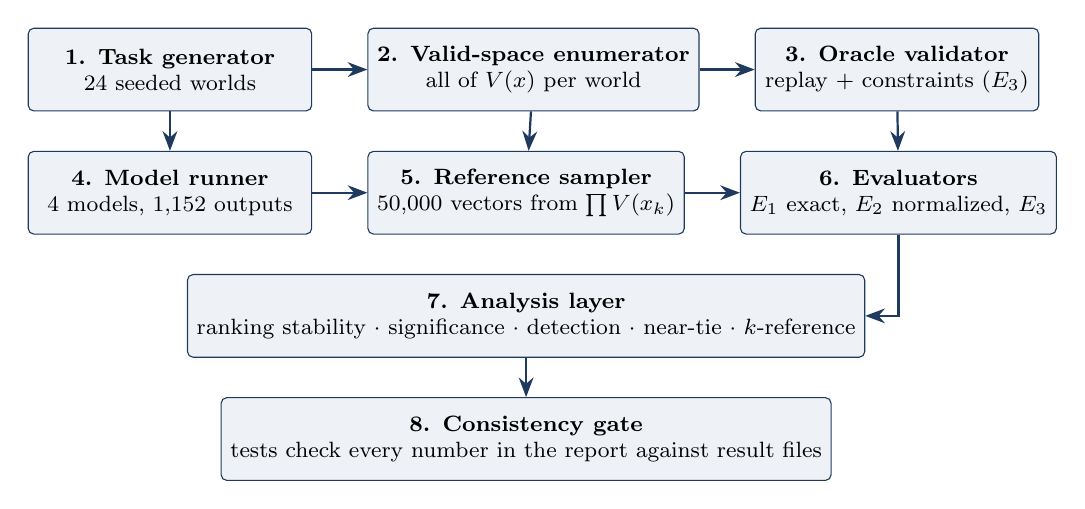
\begin{tikzpicture}[
  node distance=5mm and 7mm,
  box/.style={draw=accent,fill=soft,rounded corners=2pt,minimum width=3.6cm,minimum height=1.05cm,align=center,font=\footnotesize},
  arr/.style={-{Stealth[length=2.5mm]},thick,accent}]
\node[box] (w) {\textbf{1. Task generator}\\24 seeded worlds};
\node[box,right=of w] (v) {\textbf{2. Valid-space enumerator}\\all of $V(x)$ per world};
\node[box,right=of v] (o) {\textbf{3. Oracle validator}\\replay + constraints $(\E3)$};
\node[box,below=of w] (g) {\textbf{4. Model runner}\\4 models, 1,152 outputs};
\node[box,right=of g] (r) {\textbf{5. Reference sampler}\\50,000 vectors from $\prod V(x_k)$};
\node[box,right=of r] (e) {\textbf{6. Evaluators}\\$\E1$ exact, $\E2$ normalized, $\E3$};
\node[box,below=of r,minimum width=7.2cm] (a) {\textbf{7. Analysis layer}\\ranking stability $\cdot$ significance $\cdot$ detection $\cdot$ near-tie $\cdot$ $k$-reference};
\node[box,below=of a,minimum width=7.2cm] (c) {\textbf{8. Consistency gate}\\tests check every number in the report against result files};
\draw[arr] (w)--(v); \draw[arr] (v)--(o);
\draw[arr] (w)--(g); \draw[arr] (v)--(r); \draw[arr] (g)--(r); \draw[arr] (r)--(e);
\draw[arr] (o)--(e);
\draw[arr] (e) |- (a.east); \draw[arr] (a)--(c);
\end{tikzpicture}
\end{center}

\begin{itemize}
\item \textbf{Task generator:} produces the 24 parametric worlds; seeds make them reproducible.
\item \textbf{Valid-space enumerator:} lists every correct trajectory. The Banker's family uses a separate state-transition enumerator, cross-checked against brute-force permutation search on all 8 specifications.
\item \textbf{Oracle validator ($\E3$):} replays a candidate step by step and checks the constraints. It never reads a reference, so its verdict cannot depend on which reference was chosen.
\item \textbf{Model runner:} prompts each model over worlds, variants and seeds; outputs are frozen so every later analysis sees identical text.
\item \textbf{Reference sampler:} draws benchmark-level reference vectors (uniform, curator-biased and similarity-biased variants).
\item \textbf{Evaluators:} the three scoring rules compared in Section~\ref{sec:theory}.
\item \textbf{Analysis layer:} computes all metrics over all 50,000 draws at once, with a shared set of sign-flip permutations.
\item \textbf{Consistency gate:} a 400+ test suite and a 44-claim manifest that fail the build if any reported figure drifts from the result files.
\end{itemize}

\textbf{Design principles}
\begin{itemize}
\item Freeze generations first, then vary only the reference, so any change is attributable to reference choice alone.
\item Enumerate $V(x)$ exactly, so the ground-truth ranking is known and not estimated from human judgments.
\item Keep the oracle independent of references and (for Banker's) independent of the solver that generated the task.
\end{itemize}

% =====================================================
\subsection{Theory Behind the Method}\label{sec:theory}
\subsubsection{Valid-solution space}
\begin{itemize}
\item $V(x)$ is the set of all trajectories that obey the system's transition rules and the task's constraints.
\item In concurrency, independent events can be interleaved in many orders that all behave the same (equivalence classes of interleavings, Mazurkiewicz traces). Ties in scheduling and safe sequences in Banker's behave similarly.
\item A benchmark that stores a single answer silently treats one member of $V(x)$ as the only truth.
\end{itemize}

\subsubsection{Reference vector}
\begin{itemize}
\item For $N$ tasks, a benchmark's reference is one element of the product $V(x_1)\times\dots\times V(x_N)$.
\item This product is the ``space of possible benchmarks'' differing only in gold choice. Sampling from it turns reference choice into a controlled experimental factor.
\end{itemize}

\subsubsection{The three evaluators}
\begin{itemize}
\item $\E1$ \textbf{exact match:} output must equal the reference text (after whitespace squashing). Strictest.
\item $\E2$ \textbf{normalized match:} output must equal the reference after reducing to a canonical schedule or event trace.
\item $\E3$ \textbf{executable validator:} output passes if it is valid, whatever the reference. Treated as ground truth, so it has zero reference dependence by construction.
\end{itemize}

\subsubsection{Metrics}
\begin{itemize}
\item \textbf{Model score:} mean pass rate over worlds.
\item \textbf{Kendall $\tau_b$:} rank agreement between the ranking under a sampled reference and under the canonical one; the $b$ variant handles ties.
\item \textbf{Winner reversal:} probability that two independent reference draws give opposite winners for a model pair.
\item \textbf{$\E3$-ranking recovery:} share of draws where an evaluator reproduces the oracle's ordering exactly.
\item \textbf{Detection:} does the evaluator find the differences the oracle finds, under a proper significance test?
\item \textbf{Evaluator effect on a gap:} oracle gap minus matched-evaluator gap, with a world-level bootstrap interval.
\end{itemize}

\subsubsection{Why single references lose signal (attenuation law)}
\begin{itemize}
\item A valid output equals exactly one member of $V(x)$ and an invalid output equals none.
\item A random reference therefore accepts a valid output with probability $1/|V(x)|$.
\item Consequence: $\mathbb{E}[\E2]=\E3/|V(x)|$ for every task--model cell.
\item The share of a model gap that survives is the oracle-gap-weighted average of $1/|V(x)|$, which is predictable from solution-space sizes before any model runs.
\item The law relies on the one-match property and would fail where distinct references normalize to the same thing.
\end{itemize}

\subsubsection{Significance testing}
\begin{itemize}
\item \textbf{World-level paired sign-flip test:} per-world score differences between two models have their signs randomly flipped 20,000 times to build a null distribution. It avoids assuming normality and respects the nesting of seeds and variants.
\item \textbf{Holm--Bonferroni correction} across the 6 model pairs controls false positives from multiple comparisons.
\item The test is run on all 50,000 reference draws, giving a full distribution of decisions: significant for A, significant for B, or not significant.
\end{itemize}

\subsubsection{Remedies analysed}
\begin{itemize}
\item \textbf{Match-any with $k$ references:} an output passes if it equals any of $k$ sampled references. At $k=|V(x)|$ this equals $\E3$.
\item \textbf{Inverse-$|V|$ correction (Horvitz--Thompson style):} rescales a single-reference score by $|V(x)|$. This removes bias but leaves very large variance, so power is not restored.
\item \textbf{Executable validator:} enumerate $V(x)$ and replay candidates. Cleanest option when a validator can be written.
\end{itemize}

% =====================================================
\section{Metrics, Results and Discussion}
\subsection{Headline numbers}
\begin{center}\small
\begin{tabular}{@{}lcccc@{}}
\toprule
Evaluator & Kendall $\tau_b$ & Winner reversal & $\E3$ recovery & Mean score range\\
\midrule
$\E1$ exact & $0.769\pm0.301$ & 4.66\% & 2.86\% & 0.0--1.9\%\\
$\E2$ normalized & $0.618\pm0.351$ & \textbf{17.56\%} & 13.63\% & 0.5--4.1\%\\
$\E3$ validator & $1.000$ & 0\% & 100\% & 6.6--30.9\%\\
\bottomrule
\end{tabular}
\end{center}
\begin{itemize}
\item $\E3$ scores: \texttt{qwen3} 30.9\%, \texttt{gemma2} 17.0\%, \texttt{mistral} 7.6\%, \texttt{llama3.1} 6.6\%. All models are weak, so the whole study sits in a low-accuracy regime.
\item $\tau_b$ for $\E2$ uses 49,913 draws; 87 draws (0.17\%) have an undefined $\tau_b$ and are excluded.
\item Under the single canonical reference, $\E2$ reproduces the oracle ordering exactly. The instability only appears when other valid references are used.
\end{itemize}

\subsection{Detection of real differences}
\begin{center}\small
\begin{tabular}{@{}lccccc@{}}
\toprule
Pair & $\E3$ gap & $\E2$ gap & Gap kept & $\E3$ Holm $p$ & $\E1$/$\E2$ miss it\\
\midrule
llama3.1 vs qwen3 & $-0.243$ & $-0.037$ & 15\% & 0.013 & 100\% / 99.99\%\\
mistral vs qwen3 & $-0.233$ & $-0.037$ & 16\% & 0.018 & 100\% / 99.99\%\\
gemma2 vs qwen3 & $-0.139$ & $-0.024$ & 18\% & 0.200 & n.s.\\
gemma2 vs llama3.1 & $+0.104$ & $+0.012$ & 12\% & 0.200 & n.s.\\
gemma2 vs mistral & $+0.094$ & $+0.012$ & 13\% & 0.200 & n.s.\\
llama3.1 vs mistral & $-0.010$ & $0.000$ & $-2$\% & 0.795 & n.s.\\
\bottomrule
\end{tabular}
\end{center}

\subsection{Key results}
\begin{itemize}
\item \textbf{Reference choice alone destabilizes rankings.} $\E2$ flips a pairwise winner in 17.6\% of reference pairs.
\item \textbf{Curator bias helps but does not fix it.} Reversal falls to 12.1\% (canonical chosen 50\% of the time), 7.4\% (80\%), 2.3\% (95\%). Similarity-weighted sampling stays at 17.0\%.
\item \textbf{The larger failure is lost detection.}
  \begin{itemize}
  \item The oracle finds \texttt{qwen3} better than \texttt{llama3.1} and \texttt{mistral} under every reference.
  \item $\E1$ and $\E2$ miss both differences in 100\% and 99.99\% of draws, keeping only 15--16\% of the gap.
  \item No wrong-direction significant result occurs: the loss is power, not sign.
  \end{itemize}
\item \textbf{Near-ties dominate reversals.} 85.6\% of $\E2$ reversal mass is in pairs the oracle cannot separate (22.1\% reversal there vs 7.4\% in separated pairs).
\item \textbf{By family:} Banker's 21.0\%, synchronization 10.0\%, scheduling 0\% (uninformative, since three of four models solve none).
\item \textbf{Stating the tie-break rule does not help.} 62.5\% of semantically valid outputs are still rejected; \texttt{gemma3:12b} gives 61.9\% ($n_{\text{valid}}=42$).
\item \textbf{Adversarial set:} $\E1$/$\E2$ reject 100\% of valid-but-noncanonical answers; $\E3$ accepts them (this is true by definition of $\E3$, so it is a stress test and not an error-rate estimate).
\end{itemize}

\subsection{Remedy results (match-any with $k$ references)}
\begin{center}\small
\begin{tabular}{@{}lccccc@{}}
\toprule
$k$ & 1 & 5 & 10 & 25 & all ($\E3$)\\
\midrule
Detect qwen3 $>$ llama3.1 & 0\% & 48\% & 58\% & 84\% & 100\%\\
Detect qwen3 $>$ mistral  & 0\% & 57\% & 79\% & 88\% & 100\%\\
\bottomrule
\end{tabular}
\end{center}
\begin{itemize}
\item False positives on non-separated pairs stay near or below the nominal 5\%.
\item The inverse-$|V|$ correction reaches only 40\% / 31\% at $k=10$, below match-any (58\% / 79\%).
\end{itemize}

\subsection{Discussion}
\begin{itemize}
\item Single-gold matching in multi-solution domains mostly \textbf{hides real differences} and \textbf{makes weak orderings arbitrary}; it rarely reorders strong ones.
\item The attenuation law explains why: each valid answer survives only $1/|V(x)|$ of the time.
\item The executable validator removes the dependence by construction; the study's value is measuring the cost of not using one.
\item Scope: one 24-world benchmark, four sub-10B models, so findings are a case study and not a general claim.
\end{itemize}

% =====================================================
\section{What Went Wrong}
\begin{itemize}
\item \textbf{Wrong significance claim.}
  \begin{itemize}
  \item An early cell-level McNemar test treated seeds and variants as independent (pseudoreplication) and reported ``50\% significance flips''. Replaced by the world-level test.
  \item A later summary, ``no pair is significant'', was true only for $\E1/\E2$; $\E3$ separates two pairs. Fixed by rerunning all 50,000 draws per evaluator.
  \end{itemize}
\item \textbf{Bad citations.} Three arXiv IDs pointed to unrelated papers and one title/author list was wrong. All references were re-verified and a test now blocks mismatches. ``First'' and ``genuinely new'' claims were removed because ranking instability under reference changes is already published.
\item \textbf{Benchmark leak.} The first trace bank let a distance-to-reference classifier separate valid from invalid traces (0.663 vs a 0.65 limit); it was redesigned before any model ran. Two parser bugs were fixed after reading real outputs.
\item \textbf{Scoring-rule bug.} The analysis code omitted the rule that outputs naming outside entities never match, so 7 \texttt{mistral} outputs were wrongly counted. Fixing it moved $\tau_b$ from 0.490 to 0.618, reversal from 18.61\% to 17.56\% and recovery from 23.92\% to 13.63\%. All results were regenerated and the change is disclosed.
\item \textbf{Weak models, small benchmark.}
  \begin{itemize}
  \item Models solve only 7--31\% of tasks, so most pairs cannot be separated.
  \item The pilot's own pre-specified verdict was CONDITIONAL, and its follow-up conditions (models $\ge$50\% valid, $\ge$65 worlds) were not met.
  \item The RCR metrics are a post-hoc reanalysis, and the ``preregistration'' was an internal freeze, not an external registration.
  \end{itemize}
\item \textbf{Smaller slips:} a 200-draw significance subsample (superseded) and 87 draws with undefined $\tau_b$ that must be excluded.
\end{itemize}

% =====================================================
\section{Alternative Flow (Improvements)}
\begin{enumerate}
\item \textbf{Done: explain the effect.} Attenuation law $\mathbb{E}[\E2]=\E3/|V(x)|$ matched observations with $r=1.000$ over 42 task--model cells.
\item \textbf{Done: $k$-reference evaluation.} Detection reaches 84--88\% at $k=25$.
\item \textbf{Done: bias correction test.} Inverse-$|V|$ scaling is unbiased but too noisy.
\item \textbf{Next: more statistical power.} At least 65 worlds and 10+ models, including stronger ones, so more pairs become separable.
\item \textbf{Next: second domain.} Topological orderings of dependency graphs have exactly countable $|V|$ and would test generality.
\item \textbf{Next: LLM judges.} Check whether reference-guided judges show the same sensitivity to reference swaps.
\item \textbf{Next: external registration.} Publish the follow-up plan with an independent timestamp before running it.
\end{enumerate}

\end{document}
